\section{Complex Event Process}\label{cep}


\subsection{Zielsetzung}
Das Ziel der Anwendung ist es, die Daten welche an die MOM gesendet wurden auszulesen und dann weiterzuverarbeiten. Dabei wird mithilfe einer Complex Event Processing Engine dann nach besonderen Ereignissen gesucht. Sollte ein solches eintreffen wird eine Warnung an alle Clients über ein besonderes Topic gesendet. Die Anwendung soll sich dabei ein die 12 Faktoren einer Cloud Anwendung halten. Ein weiteres Ziel ist, dass die Anwendung in jeder Cloud laufen kann und nicht abhängig von einer bestimmten Cloud ist. 

\subsection{Umsetzungsentscheidungen}
Als Complex Processing Engine wurde Esper ausgewählt. Da Esper eine Java API besitzt und die MOM ebenenfalls über eine Javaschnittstelle verfügt (siehe Kapitel \ref{rabbitmq}) kann Esper leicht mit den anderen Komponenten der Anwendung verbunden werden. Esper besitzt zudem eine ausführliche Dokumentation, was die Umsetzung deutlich erleichtert hat. Es gibt neben Esper andere Engines welche ebenfalls mit Java verbunden werden können. Eine davon ist Apache Spark. Spark wird von Amazon direkt unterstützt und ist eine eigene Engine, welche nur noch mit Statements befüllt werden muss. Wir haben uns aber gegen Spark entschieden, da es zum einen uns stärker an die Amazon Cloud binden würde und zum anderen die Amazon Spark Engine sehr viel abnimmt und so Kontrolle über das Verhalten der Anwendung nimmt. 
\\
Die Anwendung wurde mit Java geschrieben, da es mit Java leicht ist die verschiedenen Komponenten der Anwendung zu verbinden. Java kann überall laufen, sofern eine JVM vorhanden ist. Dadurch haben wir sichergestellt, dass die Anwendung auf jeder Cloud laufen kann. Zusätzlich ist Java die Programmiersprache in der unsere Gruppe die meiste Erfahrung besitzt.   

\subsection{Esper}
Esper ist eine CEP Engine welche von EsperTech entwickelt wurde. Esper ist eine Open Source Anwendung. Eine kommerzielle Lizenz wird nur benötigt, wenn die Anwendung weiterverkauft werden soll. Esper arbeitet mit Statements, Listener und Consumption Modes. Esper speichert die eingehenden Events in einer eigenen Datenbank ab und löscht diese von selbst wenn sie nicht mehr benötigt werden. Espers Datenbank wird beim abschalten der Anwendung gelöscht. Esper ist in der Lage verschiedene unabhängige Engines gleichzeitig laufen zu lassen. 
\\ 
Die Statements basieren auf SQL. Es ist möglich Statements mit Listenern zu verknüpfen. Zusätzlich wird der Consumption Mode über die Statements angegeben. Statements können auch verwendet werden um einen Kontext anzugeben. Das wird aber in dieser Anwendung nicht benötigt, daher wird darauf nicht näher eingegangen. In einem Statement wird immer angegeben was genau gesucht wird, woher es kommen soll und was für Filterbedingungen vorhanden sind. Dabei kann in der from-Klausel auch ein Muster stehen. So kann Esper für die Mustererkennung verwendet werden. Die Statements werden auf jedes Event im Eventstrom angewendet. Sollte ein Statement zutreffen wird der dazugehörige Listener aufgerufen. Dieser kann auf die ausgewählten Werte zugreifen. Der Listner kann selbst eigene Events absenden. Der Consumption Mode legt fest ob ein weiterer Listener auf das Event zugreifen kann. Es kann auch festgelegt werden ob ein Längen- oder Zeitfenster die Zahl der zu berücksichtigen Events einschränken soll.   

\subsection{Umsetzung}
Die Anwendung wird von der InformationLifeFlow Klasse gesteuert. Diese stellt die Main-Klasse der Anwendung dar und ließt beim Start die Postleitzahlen der Städte aus. Danach wird eine Verbindung zu einer MOM erstellt. Für jede Postleitzahl wird ein sogenannter MoMReader erstellt. Diese sind eigene Threads welche für ein bestimmtes Topic auf eingehende Nachrichten warten. Der MoMSender ist das Gegenstück dazu. Der Sender sendet Nachrichten zurück zur MOM, damit diese von Clients gelesen werden können. Das Klassendiagramm zeigt die Methoden von der Mainklasse und dem Reader.
\begin{figure}[htbp]
	\centering
	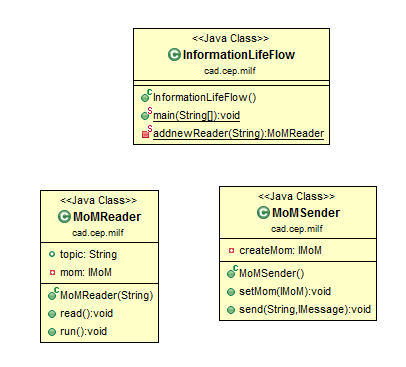
\includegraphics[width=0.5\textwidth]{Bilder/FlowAndReader.png}
	\caption{Klassendiagramm der Steuerungsklassen}
	\label{img:flowDiagramm}
\end{figure} 
Die MOM wird mithilfe einer Factory Klasse erstellt. Diese erstellt beim ersten Aufruf eine Verbindung zur MOM und gibt diese bei jeden Aufruf wieder zurück. Derzeit unterstützt die Anwendung nur eine MQTT-MOM. Mithilfe des IMoM Interfaces kann aber jederzeit eine weitere MOM hinzugefügt werden. Die MQTT MOM benötigt einen Hostpfad, einen Usernamen und ein Passwort. Diese werden von der Factory aus den Umgebungsvariablen ausgelesen und dann der MOM weitergegeben. Die MOM öffnet eine Verbindung und ist danach in der Lage Nachrichten zu senden oder zu Empfangen. Jede empfangene Nachricht wird von einer Callback-Methode ausgewertet. Diese überprüft was für ein Typ die Nachricht besitzt und behandelt diese dann entsprechend. Das bedeutet ein Forcast wird umgeformt und weitergeleitet während eine Tagesmeldung weiter an die CEP Engine gesendet wird. Beim Umformen des Forcasts wird auch die maximale Temperatur, die minimale Temperatur und das Durchschnittswetter für jeden Tag ermittelt. Das folgende Klassendiagramm zeigt die Komponenten der MOM-Verbindung.
\begin{figure}[htbp]
	\centering
	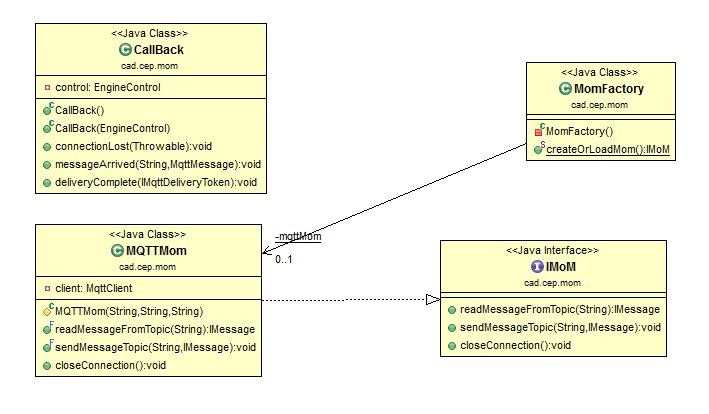
\includegraphics[width=0.5\textwidth]{Bilder/MoMKomponents.png}
	\caption{Klassendiagramm der MOM Komponenten}
	\label{img:MoMDiagramm}
\end{figure} 
Die Anwendung kennt verschiedene Nachrichtentypen. Die Nachrichten die eingehen sind entweder eine Nachricht vom Typ "JSONMessage" oder vom Typ "WeeklyForcast". Die JSONMessage stellt dabei die Nachricht für den aktuellen Wetterstand dar. Das sind die häufigsten Nachrichten die eingehen. Wie der Name schon andeutet, kommen die Nachrichten in einen JSON-Format an, dass direkt mithilfe von GSON in eine Instanz der Klasse umgeformt wird. Die WeeklyForcast Nachrichten kommen zwar auch in einem JSON-Format an, müssen aber nochmal umgewandelt und gefiltert werden, bis die benötigte Nachricht entsteht. Diese Nachrichten kommen deutlich seltener bei der Anwendung an da diese einen Abschätzung der nächsten Tage darstellt. Die JSONMessage wird zur weiteren Auswertung an die CEP Engine übergeben. Der Wochenbericht wird direkt weiterverarbeitet. Im folgenden Klassendiagramm werden die Nachrichten mit ihren Methoden gezeigt. 
\begin{figure}[htbp]
	\centering
	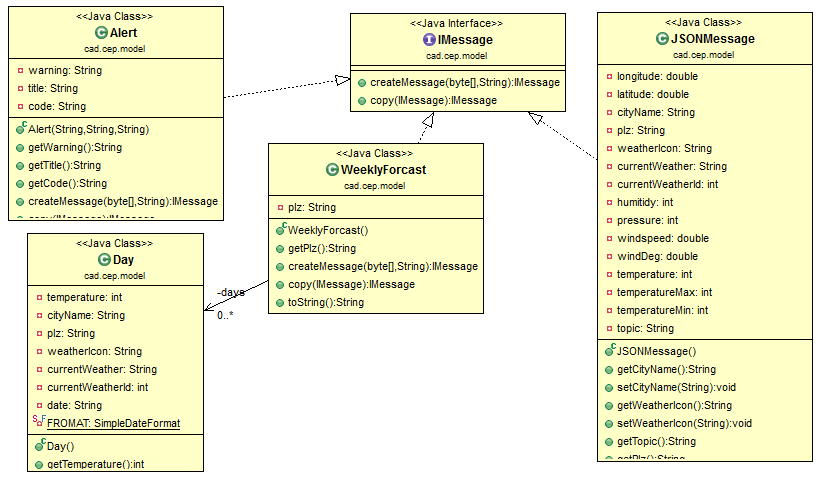
\includegraphics[width=0.5\textwidth]{Bilder/News.png}
	\caption{Das Klassendiagramm der Nachrichten}
	\label{img:eventDiagramm}
\end{figure} 
Sollte die CEP Engine etwas finden wird ein Alert gesendet. Diese Nachrichten beinhalten einen Titel, eine Warnung und einen Warnungscode. Der Title kann verwendet werden um herauszufinden worüber gewarnt wird, die Warnung selbst ist der englische default Text und der Code kann verwendet werden um die Warnung in eine andere Sprache zu übersetzen.  Die Folgende Tabelle zeigt die Warnungscodes. 
\begin{table}[!ht]
  \centering
    \begin{minipage}{15cm}
      \centering
      \begin{tabular}{*{3}{|l|p{5.0cm}|p{5.0cm}}}\hline
      \multicolumn{4}{|c|}{\cellcolor[RGB]{200,200,200}Die Warnung-Codes} \\\hline
     \textbf{Code}&\textbf{Bedeutung}\\\hline
    T1&Tropisches Wetter: Luftfeuchtigkeit über 90\\
      \hline
     W1&Forstchance: Es kann sein das es Frost auf der Straße gibt\\
     \hline
     W2&Starke Kälte: Die Temperatur ist unter -9 Grad\\
     \hline
     W3&Starker Schneefall: Besonders heftiger Schneefall\\
     \hline 
     S1&Gutes Wetter: Es scheint die Sonne und es hat über 25 Grad\\
     \hline
      H1&Herzinfakt Warnung: Für Herzkranke starke Luftdruck Schwankungen\\
     \hline
      H2&Herzinfakt Warnung: Für Herzkranke zu hohe Temperatur (>=25)\\
     \hline
      \end{tabular}
   \caption{Die Wanung-Codes}\label{tab:WaningCodes}
    \end{minipage}
\end{table}
Die CEP Engine wird über die Klasse Engine Control gesteuert. Diese Singleton-Klasse stellt sicher, dass die anderen Klassen Zugriff auf von ihnen benötigten Funktionen der Engine haben, aber dabei nicht mehr Zugriff als notwendig erhalten. Die Klasse ist ein Singleton um sicherzugehen das jede Klasse auf die gleiche Engine zugreift. Die Klasse selbst erstellt eine Instanz der Klasse EsperService. Die Instanz wrid über eine Factory erstellt. Die Factory geht sicher das jedes benötigte Statement mit einen Listener verknüpft wird. Die EsperService-Klasse beinhaltet die tatsächliche Esper Engine und stellt einen Wrapper für diese dar. Das folgende Klassendiagramm zeigt die Methoden und die Abhängigkeiten der Klassen.
 \begin{figure}[htbp]
	\centering
	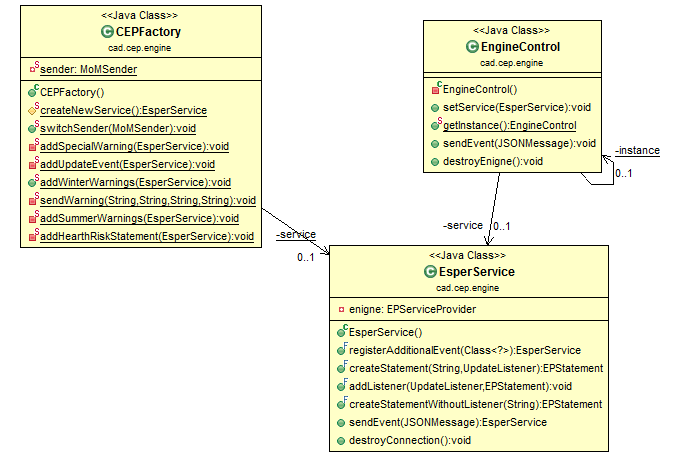
\includegraphics[width=0.5\textwidth]{Bilder/Esper.png}
	\caption{Das Klassendiagramm der CEP Klassen}
	\label{img:esperDiagramm}
\end{figure} 
Die Esper Statements sorgen dafür, dass Muster in den eingehenden Wetterdaten erkannt werden, und reagieren mit passenden Nachrichten auf diese. Die Statements werden von der CEPFactory der Engine hinzugefügt. Jede eingehende Nachricht wird von mindestens einem Statement erfasst. Der entsprechende Listener sorgt dafür, dass die Clients die Daten erhalten und gibt eine Ausgabe aus. Zusätzlich werden die Daten in der Datenbank gespeichert. Dabei gibt es kein Fenster oder Consumption Mode (TODO Was wie wo willst du damit sagen??? Gleicher Satz ein Absatz drunter nochmal). Jede Nachricht wird von diesem Statement erfasst und es dürfen auch weitere Statements greifen. Das Statement sieht wie folgt aus: 
\begin{lstlisting}
select * from JSONMessage
\end{lstlisting}
Ein weiteres Statement prüft ob die Luftfeuchtigkeit zu hoch ist. Bei einer hohen Luftfeuchtigkeit liegen tropische Verhältnisse vor, welche in Deutschland eher ungewöhnlich wären. Da alle unsere Wetterdaten aus Deutschland stammen ist es daher wichtig die Clients über eine solche Besonderheit zu informieren. Auch dafür gibt es kein Fenster und keinen Consumption Mode (TODO). Treten die Bedingungen ein, liegt also eine Luftfeuchtigkeit von über 90\% vor, wird ein Alert gesendet. Es dürfen aber auch andere Ereignisse ausgewertet werden.  Die Nachricht erhält den Code T1. 
\begin{lstlisting}
select * from JSONMessage where humidity >= 90
\end{lstlisting}
Einige Warnungen sind vor allem im Winter wichtig. Dabei geht es um Schneefall, niedrige Temperaturen und Frost. Die erste Winternachricht W1 warnt über eine Frostgefahr. Dabei werden zwei JSONMessages ausgewertet, ob sie nacheinander ins System gekommen sind, dabei aus dem gleichen Ort stammen und Temperaturen unter 0 Grad angeben. Es werden zwei aufeinander folgende Nachrichten benötigt, da Wasser nicht sofort gefriert sondern Zeit braucht. Wenn also zwei Messungen eine negative Temperatur angeben, hatte das Wasser Zeit zu gefrieren. Sollte auf eine Nachricht mit negativer Temperatur eine Nachricht mit positiver Temperatur oder 0 Grad folgen, wird davon die erste Nachricht entfernt da das Wasser nicht genug zeit zum gefrieren hatte. Das Statement sieht wie folgt aus: 
\begin{lstlisting}
select * from pattern[m1=JSONMessage ->
m2=JSONMessage
(m1.plz = m2.plz and m1.temperature <0 and m2.temperature <0]
\end{lstlisting}
Über die Identifier m1 oder m2 können die einzelnen Nachrichten im Listener angesprochen werden. Der Listener sendet die Nachricht wieder als Alert weiter. W2 ist die zweite Nachricht und gibt eine Meldung bei besonderst kalten Temperaturen aus. Dabei benötigt es nur eine Nachricht mit einer Temperatur von unter -9 Grad um eine Warnung auszugeben. Niedirgere Temperaturen sind normalerweise selten in Deutschland und generell eher gefährlich. Daher muss eine Warnung an die Clients weitergeben werden. Das Statement funktioniert wie die bereits beschriebenen Statements. 
\begin{lstlisting}
select * from JSONMessage where temperature <=-9
\end{lstlisting}
Die Letzte Winternachricht befasst sich mit starken Schneefall. Dabei wrid der Wettercode von der Wetterapi ausgewertet. Der Code 622 bedeutet starker Schneefall. Die Clients können den Code zwar auswerten und auch entsprechend Meldungen ausgeben aber starker Schneefall kann gefährlich werden. Daher wird eine Meldung weitergesendet um sicherzugehen das alle Clients auch ihre Nutzer warnen. Das Statement sieht wie folgt aus. 
\begin{lstlisting}
select * from JSONMessage where currentWeatherId = 622
\end{lstlisting}  
Für den Sommer gibt es eine eigene Warnung. Diese warnt den Nutzer vor sehr guten Wetter. Das ist normalerweise nicht gefährlich aber es kann Clients interessieren ob sie ihren Nutzern sagen können, dass diese Baden gehen können. Dabei wurden als Bedingungen eine Temperatur über 25 Grad und ein klarer Himmel verwendet. Die ID dieses Alarms ist S1. 
\begin{lstlisting}
select * from JSONMessage where temperature > 25 and currentWeatherId >= 800
\end{lstlisting}
Die letzte Warnungskategorie beschäftigt sich mit Herzinfaktrisiken. Die Anwendung ist keine Medizinische Anwendung und folgt auch nicht den denentsprechenden Richtlinien. Daher kann die Anwendung nicht eine genaue Aussage darüber treffen ob ein Herzkranker Tabletten nehmen muss. Die Anwendung kann aber Aussgaben darüber treffen was laut Statistiken gefährlich für Menschen mit Herzproblemen werden könnte. Das stellt aber keine Empfehlung Medikamente zu nehmen dar. Es soll die Nutzer nur darauf hinweisen das sie sich Gedanken machen sollten, ob sie davon betroffen werden können. 
 Schwankt der Luftdruck zu strark, kann bei einigen Menschen es zu einen Herzinfakt kommen. Daher gibt es ein Statement welches überprüft ob in den letzten 30 Minuten eine starke Schwankung stattgefunden hat. Wenn eine Meldung in den Eventstream gelangt wird diese aufbewahrt bis das Zeitfenster abgelaufen ist oder das Muster erkannt wurde. Das Statement sieht wie folgt aus:

\begin{lstlisting}
select * from pattern[d1=JSONMessage ->
d2=JSONMessage
(p1.plz = p2.plz and
 (p2.pressure - p1.pressure <-5 or 
p1.pressure - p2.pressure <-10))
 where timer:within(30 min)]
\end{lstlisting} Das Statement W2 beschäftigt sich mit der Gefahr einer zu hohen Temperatur. Sollte diese über 25 Grad sein kann es in eingien Fällen das herzinfaktrisiko erhöhen. Das Statement dazu entspricht den anderen Updatestatements. 

\begin{lstlisting}
select * from JSONMessage wgere temperature >=25
\end{lstlisting}
 Zu jeden Eintrag in der Tabelle \ref{tab:WaningCodes} gibt es ein eigenes Statement. Dazu gibt es ein Statement um jede Nachricht zu erfassen. Dabei werden keine unique Consumptionmodes verwendet da eine Nachricht mehrere Statements auslösen kann. Es kann zum Beispiel gutes Badewetter, ein hoher Luftddruck und eine hohe Luftfeuchtigkeit gleichzeitig eintreten. Genauso wie eine Nachricht nicht im Eventstream bis zum erreichen eines Fensterendes oder eines Musters blockiert werden kann. Während die erste Nachricht darauf wartet wegen der temperatur Schwankungen festgehalten zu werden, kann eine andere Nachricht eingehen die in Kompination mit der ersten Nachricht ein anderes Muster erfüllt.  
\subsection{Ablauf}
Sobald die Anwendung gestartet wurde, ließt diese alle ihr bekannten Städte aus. Für jede Postleitzahl werden zwei Reader-threads erstellt. Einer davon wartet auf alle Nachrichten unter den Topic plz/today und der andere wartet auf alle Nachrichten unter dem Topic plz/weekly. Damit der Reader die Nachrichten auch erhält muss eine Verbindung zur MoM erstellt werden. Dafür wird die Adresse und die Credentials für die MoM aus den Umgebungsvariablen ausgelesen. Die Nachrichten kommen in einen JSON Format an. Dieses Format wird versucht in eine Instanz der Klasse JSONMessage umzuwandeln. Klappt das nicht wird verscuht daraus eine WeeklyForcast Nachricht zu machen. Klappt das auch nicht gibt die Anwendugn eine Fehlermeldung aus und ignoriert die Nachricht, Jede JSONMessage wird als Event den Eventstream der CEP weitergegeben. Sollte die Engine eine Besonderheit finden wird eine Warnung an plz/alert gesendet. Auf jedenfall wird die Nachricht an plz/today/cep weitergeleitet. Die Wochenvorhersage wird an plz/weekly/cep gesendet.  
\subsection{Erfüllte Anforderungen}
Die Anwendung muss sich natürlich an die Anforderungen des 12-Faktor App Standards halten. Die erste Anforderung Codebase wird dadurch erfüllt das die Anwendung selbständig und alleine Funktionieren kann. Die anderen Komponenten, wie zum Beispiel die Wetter API sind nicht notwendig. Sie wurden nur mit entwickelt um ein Vollständiges Scenario darstellen zu können. Die einzige notwendige andere komponente ist eine MoM. Dabei kann die MoM aber jederzeit ausgetauscht werden. Die MoM wurde auch nicht von uns entwickelt sondern nur auf dem Server aufgesetzt. 
\\
Die Abhänigkeiten werden mit Maven verwaltet. Jede Benötigte Bibliothek wird einfach als Dependency hinzugefügt und diese wird, mit allen von dieser Benötigten Bibliotheken, runtergeladen und im Buildpath hinzugefügt. Neue Versionen oder Abhänigkeiten können einfach mit einer Zeile mehr in der Konfiguration hinzugefügt werden. Es wird nichts an Code Verwendet was nicht entweder von Java selbst kommt (Version 1.8) oder aus einer in Maven definierten Bibilothek vorhanden ist. Die Anwendung geht niemals davon aus das etwas implizit vorhanden ist.
\\
Die Addresse der MoM, der Nutzername und das Passworrt sind alle in Umgebungsvariablen festgelegt. Die einzige Konsigurationsdatei im Projekt ist die pom.xml. Diese hat aber mit der laufenden Anwendung nach dem erstellen des Builds nichts mehr zu tun. 
\\
Die Anwendung verwendet als anderen Service die MoM. Diese wird über eine API angesprochen. Die API ist allgemeingültig für jede MoM, sofern sie MQTT unterstüzt. Die Datenbank wird über eine selbstgeschriebene API angesprochen. Die Art der Datenbank kann über eine neue Klasse ausgetauscht werden, da über ein Interface die Datenbank angesprochen wird. Die Adresse kann auch ausgetauscht werden. 
\\
Der Relasebuild kann nur von Jenkins erstellt werden. Dieses erstellt alle zusätzlichen für eine veröffentlichte Version benötigten Datein. Jenkins erlangt den Code über das Github Repository. Zu den Dateien gehört unter anderen die Konfiguration für das Deployment auf der Cloud.
\\
Säntliche Daten werden nur kurzeitig von der CEP Engine gespeichert. Die Anwendung legt keine Files an welche länger als die Ausführungszeit auf dem Server vorhanden sind. Daten die nicht mehr vorhanden sind, werden auch nicht mehr aufgerufen. Die CEP kennt nur die Temporär gespeicherten Daten. jede Datei die nicht mehr gespeichert ist, wird von der Engine nicht mehr berücksichtigt. Daher wird jede eingehende Nachricht zusätzlich in einer Datenbank gespeichert. Wenn die Engine startet werden alle Daten der letzten 24 Stunden geladen und neu gesendet. Auf dieseweise gehen keine Informationen verloren.
\\
Die Anwendung braucht nur eine JVM zum Laufen. Ansonsten wird davon ausgegangen das über die Cloud Foundry oder die Cloud eines anderen Anbieters über eine Einstellung die Anwendung mit einen Port verknüpft werden kann. 
\\
Es werden verschiedene Threads verwendet. Diese werden aber nicht wegen der zum skalieren verwendet, sondern um sicherzugehen das eine Nachricht ausgewertet werden kann während eine andere gesendet wird. Es soll also nur die Ausführungszeit verschiedener nebenläufig ausführbarer Schritte optimiert werden. Weitere instanzen der Cloud werden zum skalieren erstellt. 
\\
Es macht keinen unterschied ob die Anwendung normal geschlossen wurde oder abgestürzt ist. Die CEP Engine und die MoM Verbindung werden geschlossen und können ohne Probleme wieder geöffnet werden. Wenn eine Verbindung wieder gebraucht wird, wird diese automatsich wieder geöffnet. Nur die bisherigen Muster gehen Verloren wenn die Anwendung plötzlich abstürtzt. Sobald die Anwendung neu startet werden die Daten der letzten 24 Stunden geladen und neu gesendet. Die Muster können so wiederhergestellt werden. Alles was älter als 24 Stunden ist, ist nicht mehr relevant. 
\\
Es werden keine Log-Dateien angelegt. Die Anwendug gibt Mledungen über den Output- und den ErrorStream aus. An einer anderen Stelle muss daraus ein Log oder eine sonstige Auswertung erfolgen. 
\\
In der folgenden Tabelle werden die Anforderungen nochtmal zusammengefasst dargestellt. 
\begin{table}[!ht]
  \centering
    \begin{minipage}{15cm}
      \centering
      \begin{tabular}{*{3}{|l|p{5.0cm}|p{5.0cm}}}\hline
      \multicolumn{4}{|c|}{\cellcolor[RGB]{200,200,200}Validierung nach "12 Faktor APP"} \\\hline
     \textbf{ID}&\textbf{Anforderung}&\textbf{Validierungs Element}&\textbf{Erfüllt}\\\hline
     1.&Codebase&Andere Komponenten sind nur für das Testszenario da. Deployment verschiederner Versionen über Repo möglich&Ja\\
      \hline
     2.&Abhängigkeiten&Abhängigkeiten werden über Maven verwaltet&Ja\\
     \hline
     3.&Konfiguration&Bis auf Buildconfigurations gibt es keine Konfigurationsdatei. Alles andere über Umgebungsvariablen&Ja\\
     \hline
     4.&Unterstützende Dienste&Die unterstüzenden Dienste können über Umgebungsvariablen ausgetauscht werden&Ja\\
     \hline 
     5.&Build, release, run&Wird von Jenkins verwaltet&Ja\\
     \hline
     6.&Prozesse&Es gibt keine langfristig gespeicherten Daten&Ja\\
     \hline
      7.&Bindung an Ports&Wird von Cloud Foundry übernommen&Ja\\
     \hline
      8.&Nebenläufigkeit&Es wird nicht mit threads skaliert sondern mit Cloud Foundry instanzen&Ja\\
     \hline
      9.&Einweggebrauch&Verbindungen können beliebig geschlossen oder geöffnet werden ohne das wichtige Daten verloren gehen&Ja\\
     \hline
     10.&Dev-Prod-Vergleichbarkeit&Nicht zutreffent&Nein\\
     \hline     
     11.&Logs&Es wird mit den Streams gearbeitet.&Ka\\
     \hline
     12.&Admin-Prozesse&Nicht zutreffent&Nein\\
     \hline
      \end{tabular}
   \caption{Validierung der CEP nach "12 Faktor APP"}\label{tab:AnforderungenCEP}
    \end{minipage}
\end{table}